\documentclass[11pt,letterpaper]{article}
\usepackage[lmargin=1in,rmargin=1in,tmargin=1in,bmargin=1in]{geometry}
\usepackage{../style/homework}
\usepackage{../style/commands}
\setbool{quotetype}{true} % True: Side; False: Under
\setbool{hideans}{false} % Student: True; Instructor: False

% -------------------
% Content
% -------------------
\begin{document}

\homework{5: Due 01/11}{I just want to lie on the beach and eat hot dogs. That's all I've ever wanted.}{Kevin Malone, The Office}

% Problem 1
\problem{10} Determine if the following function is linear. Explain why or why not.
	\begin{table}[!ht]
	\centering
	\begin{tabular}{c|c}
	$x$ & $f(x)$ \\ \hline
	$1.2$ & $7.16$ \\
	$2.8$ & $12.39$ \\
	$4.4$ & $16.12$ \\
	$6.0$ & $22.13$ \\
	$7.6$ & $25.08$
	\end{tabular}
	\end{table}

\sol We compute the slopes:
	\[
	\begin{aligned}
	m&= \dfrac{12.39 - 7.16}{2.8 - 1.2}= \dfrac{5.23}{1.6}= 3.26875 \\[0.3cm]
	m&= \dfrac{16.12 - 12.39}{4.4 - 2.8}= \dfrac{3.73}{1.6}= 2.33125 \\[0.3cm]
	m&= \dfrac{22.13 - 16.12}{6.0 - 4.4}= \dfrac{6.01}{1.6}= 3.75625 \\[0.3cm]
	m&= \dfrac{25.08 - 22.13}{7.6 - 6.0}= \dfrac{2.95}{1.6}= 1.84375
	\end{aligned}
	\]
Because the slope is not constant, this function cannot be linear. 



\newpage



% Problem 2
\problem{10} A linear function has a table whose values are given below. Find the equation of the linear function. Be sure to specify the slope and $y$-intercept.
	\begin{table}[!ht]
	\centering
	\begin{tabular}{c|c}
	$x$ & $f(x)$ \\ \hline
	$2$ & $20$ \\
	$7$ & $-5$ \\
	$12$ & $-30$ \\
	$17$ & $-55$
	\end{tabular}
	\end{table}

\sol Because this line is clearly not vertical, we know that $y= mx + b$. First, we compute the slope:
	\[
	m= \dfrac{-5 - 20}{7 - 2}= \dfrac{-25}{5}= -5
	\]
Now we use the fact that $(2, 20)$ is on the line:
	\[
	\begin{aligned}
	y&= mx + b \\[0.3cm]
	y&= -5x + b \\[0.3cm] 
	20&= -5(2) + b \\[0.3cm]
	20&= -10 + b \\[0.3cm]
	b&= 30
	\end{aligned}
	\]
Therefore, we have\dots
	\[
	\framebox{$y= -5x + 30$}
	\]



\newpage



% Problem 3
\problem{10} Plot the linear function $y= \frac{3}{2} x - 4$ using the ``two-point'' method. \pspace
	\[
	\fbox{
	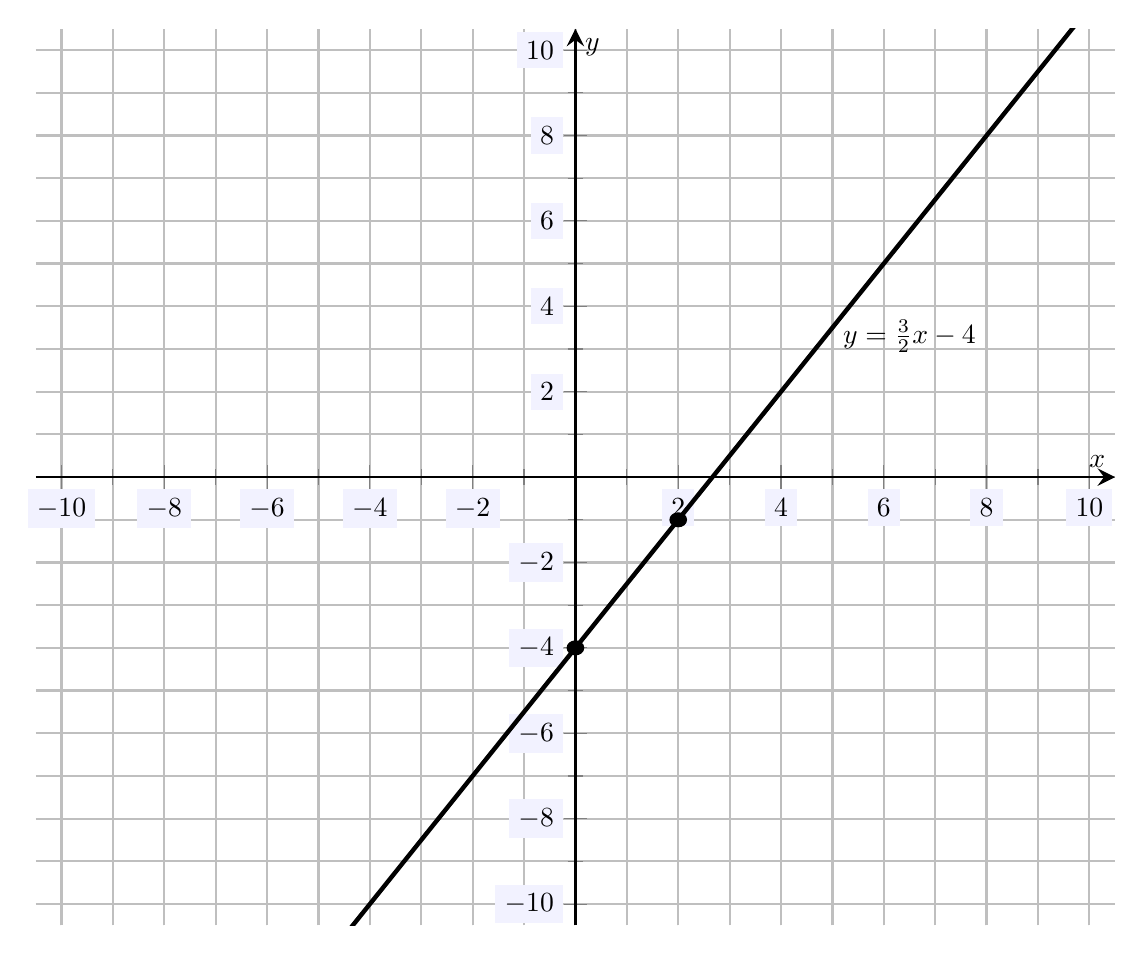
\begin{tikzpicture}[scale=2,every node/.style={scale=0.5}]
	\begin{axis}[
	grid=both,
	axis lines=middle,
	ticklabel style={fill=blue!5!white},
	xmin= -10.5, xmax=10.5,
	ymin= -10.5, ymax=10.5,
	xtick={-10,-8,-6,-4,-2,0,2,4,6,8,10},
	ytick={-10,-8,-6,-4,-2,0,2,4,6,8,10},
	minor tick = {-10,-9,...,10},
	xlabel=\(x\),ylabel=\(y\),
	]
	\node at (6.5,3.3) {$y= \frac{3}{2}x - 4$};
	\addplot[thick, domain= -10.5:10.5] ({x},{3/2*x - 4});
	\draw[fill=black] (0,-4) circle (0.15);
	\draw[fill=black] (2,-1) circle (0.15);
	\end{axis}
	\end{tikzpicture}
	}
	\] \pspace

We compute any two points on the curve. For instance, we have\dots
	\[
	\begin{aligned}
	y(0)&= \frac{3}{2} \cdot 0 - 4 = 0 - 4= -4 \rightsquigarrow (0, -4) \\
	y(2)&= \frac{3}{2} \cdot 2 - 4= 3 - 4= -1 \rightsquigarrow (2, -1)
	\end{aligned}
	\]
We can then plot these point and connect them linearly. 



\newpage



% Problem 4 
\problem{10} Plot the linear function $y= -\frac{1}{2} x + 3$ using the ``slope'' method. 
	\[
	\fbox{
	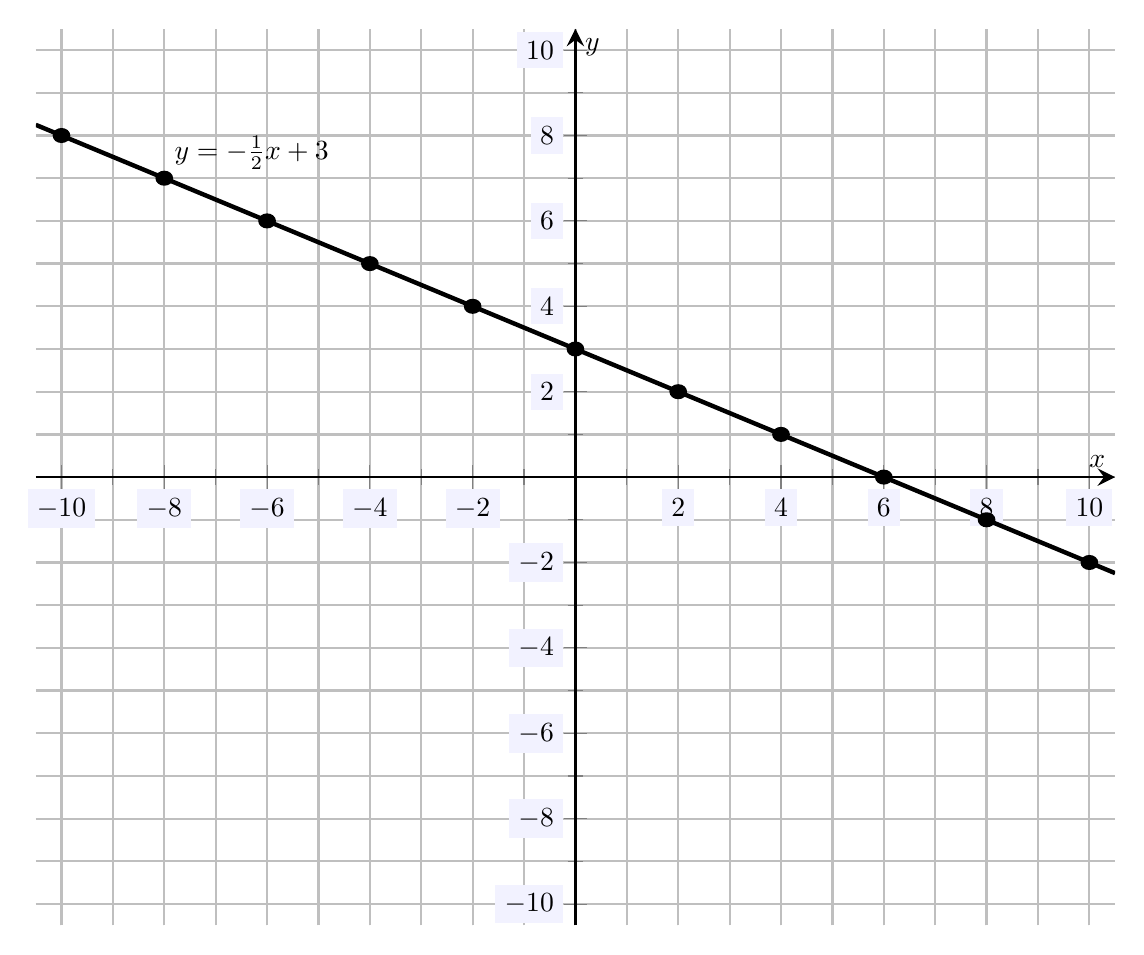
\begin{tikzpicture}[scale=2,every node/.style={scale=0.5}]
	\begin{axis}[
	grid=both,
	axis lines=middle,
	ticklabel style={fill=blue!5!white},
	xmin= -10.5, xmax=10.5,
	ymin= -10.5, ymax=10.5,
	xtick={-10,-8,-6,-4,-2,0,2,4,6,8,10},
	ytick={-10,-8,-6,-4,-2,0,2,4,6,8,10},
	minor tick = {-10,-9,...,10},
	xlabel=\(x\),ylabel=\(y\),
	]
	\node at (-6.3,7.6) {$y= -\frac{1}{2}x + 3$};
	\addplot[thick, domain= -10.5:10.5] ({x},{-1/2*x + 3});
	\draw[fill=black] (-10,8) circle (0.15);
	\draw[fill=black] (-8,7) circle (0.15);
	\draw[fill=black] (-6,6) circle (0.15);
	\draw[fill=black] (-4,5) circle (0.15);
	\draw[fill=black] (-2,4) circle (0.15);
	\draw[fill=black] (0,3) circle (0.15);
	\draw[fill=black] (2,2) circle (0.15);
	\draw[fill=black] (4,1) circle (0.15);
	\draw[fill=black] (6,0) circle (0.15);
	\draw[fill=black] (8,-1) circle (0.15);
	\draw[fill=black] (10,-2) circle (0.15);
	\end{axis}
	\end{tikzpicture}
	}
	\] \pspace

We find a point on the line. For instance, we know $y(0)= -\frac{1}{2} \cdot 0 + 3= 0 + 3= 3$, which gives the point $(0, 3)$. We know the slope is $m= -\frac{1}{2}$, which we can interpret as\dots
	\[
	\dfrac{\Delta y}{\Delta x}= \dfrac{-1}{2}= \dfrac{1}{-2}
	\]
That is, for every increase of 2 in $x$, $y$ decreases by $1$ or for every decrease in 2 in $x$ there is a corresponding increase of 1 in $y$. This yields the plot above. 



\newpage



% Problem 5
\problem{10} Suppose water is draining from a tank. The number of gallons of water in the tank $t$ hours from now is given by $W(t)= 567.8 - 24.1t$.
\begin{enumerate}[(a)]
\item Is $W(t)$ linear? Explain.
\item What is the slope of $W(t)$? Interpret the slope.
\item Explain how we can know that water is draining from the tank using (b).
\item What is the $y$-intercept for $W(t)$? Interpret this intercept. 
\item Sketch a plot of $W(t)$ and estimate when the tank will be completely empty. 
\end{enumerate} 

\sol 
\begin{enumerate}[(a)]
\item Yes. Writing $W(t)= -24.1t + 567.8$, we see that $W(t)$ has the form $mx + b$, where $x= t$, $m= -24.1$, and $b= 567.8$. Moreover, the water is draining from the tank at a constant rate so that $W(t)$ must be linear. 

\item From (a), we see that $m= -24.1$. Thinking of $-24.1$ as $\frac{-24.1}{1}$ and interpreting it as $\dfrac{\Delta y}{\Delta x}$, we see that for each increase of 1 in $x$, we see a corresponding decrease of 24.1 in $y$. In context, this slope means that each hour 24.1~gallons of water drains from the tank. 

\item Because $m < 0$, we know that $W(t)$ is decreasing. Because this represents the amount of water in the tank, we know that the amount of water in the tank is decreasing. 

\item We have $W(0)= 567.8 - 24.1(0)= 567.8 - 0= 567.8$. Therefore, the $y$-intercept is $(0, 567.8)$. This means when $t= 0$, then $W= 567.8$. We know $t= 0$ is 0~hours from now, i.e. the initial time, and that at this moment there was 567.8~gallons of water in the tank. Therefore, we can interpret the $y$-intercept as the information that the initial amount of water in the tank was 567.8~gallons. 

\item The tank is empty when $W(t)= 0$. From the plot below, we can see that the tank completely empties sometime between 22~hours and 24~hours from now. We can approximate this as 23.5~hours from now. Computing this exactly, we find the tank empties in 23.5602~hours. \par
	\[
	\fbox{
	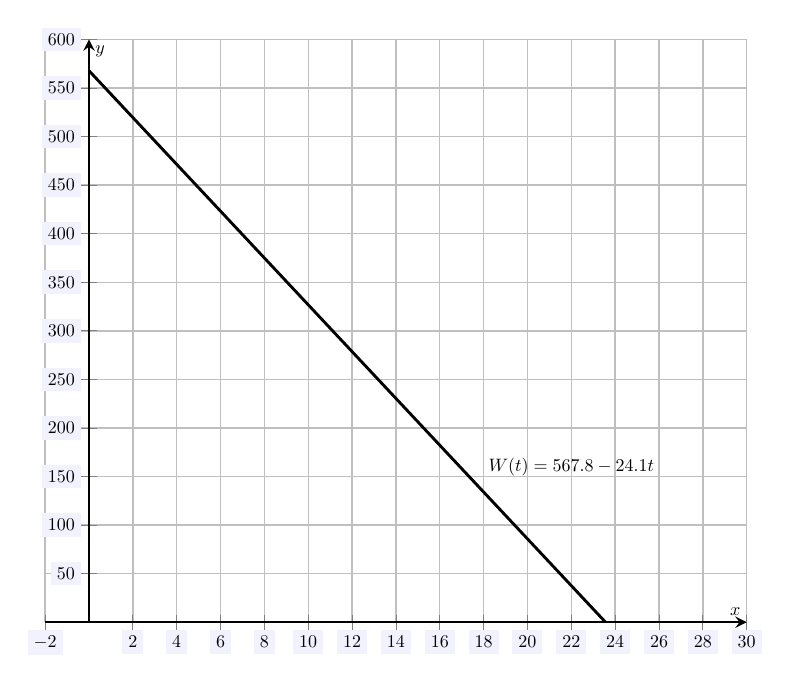
\begin{tikzpicture}[scale=1.3,every node/.style={scale=0.5}]
	\begin{axis}[
	grid=both,
	axis lines=middle,
	ticklabel style={fill=blue!5!white},
	xmin= -2, xmax=30,
	ymin= -0.10, ymax=600,
	xtick={-2,0,2,...,30},
	ytick={-10,0,50,100,...,600},
	xlabel=\(x\),ylabel=\(y\),
	]
	\node at (22,160) {$W(t)= 567.8 - 24.1t$};
	\addplot[thick, domain= 0:30] ({x},{-24.1*x + 567.8});
	\end{axis}
	\end{tikzpicture}
	}
	\] 
\end{enumerate}



\newpage



% Problem 6
\problem{10} Consider the linear equation $12x - 2y= 56$. 
\begin{enumerate}[(a)]
\item Solve the linear equation for $y$. 
\item Determine the slope and $y$-intercept for the corresponding line.
\item Interpret the slope in at least two different ways. 
\end{enumerate} \pspace

\sol
\begin{enumerate}[(a)]
\item 
	\[
	\begin{aligned}
	12x - 2y&= 56 \\[0.3cm]
	-2y&= -12x + 56 \\[0.3cm]
	y&= 6x - 28
	\end{aligned}
	\] \pspace

\item Because $y= 6x - 28$ is in the form $y= mx + b$, we know that $m= 6$, i.e. the slope is 6, and that $b= -28$, which implies that the $y$-intercept is $(0, -28)$. \pspace

\item We know that the slope is $m= 6= \frac{6}{1}$. Thinking of the slope as $\frac{6}{1}= \dfrac{\Delta y}{\Delta x}$, we can interpret this as $\Delta x= 1$ and $\Delta y= 6$. But then for every increase of 1 in $x$, we see a corresponding increase of 6 in $y$. Alternatively, thinking of the slope as $\frac{6}{1}= \frac{-6}{-1}= \dfrac{\Delta y}{\Delta x}$, we can interpret this as $\Delta x= -1$ and $\Delta y= -6$. But then for every decrease of 1 in $x$, we see a corresponding decrease of 6 in $y$.
\end{enumerate}



\newpage



% Problem 7
\problem{10} Consider the linear equation $7.6x + 14.9y= 429.1$. 
\begin{enumerate}[(a)]
\item Solve the linear equation for $y$. 
\item Determine the slope and $y$-intercept for the corresponding line.
\item Interpret the slope in at least two different ways. 
\end{enumerate} \pspace

\sol
\begin{enumerate}[(a)]
\item 
	\[
	\begin{aligned}
	7.6x + 14.9y&= 429.1 \\[0.3cm]
	14.9y&= -7.6x + 429.1 \\[0.3cm]
	y&= -0.510067x + 28.7987
	\end{aligned}
	\] \pspace

\item Because $y= -0.510067x + 28.7987$ is in the form $y= mx + b$, we know that $m= -0.510067$, i.e. the slope is $-0.510067$, and that $b= 28.7987$, which implies that the $y$-intercept is $(0, 28.7987)$. \pspace

\item We know that the slope is $m= -0.510067= \frac{-0.510067}{1}$. Thinking of the slope as $\frac{-0.510067}{1}= \dfrac{\Delta y}{\Delta x}$, we can interpret this as $\Delta x= 1$ and $\Delta y= -0.510067$. But then for every increase of 1 in $x$, we see a corresponding decrease of $0.510067$ in $y$. Alternatively, thinking of the slope as $\frac{-0.510067}{1}= \frac{0.510067}{-1}= \dfrac{\Delta y}{\Delta x}$, we can interpret this as $\Delta x= -1$ and $\Delta y= 0.510067$. But then for every decrease of 1 in $x$, we see a corresponding increase of $0.510067$ in $y$.
\end{enumerate}



\newpage



% Problem 8
\problem{10} Consider the line given by $y= -\frac{7}{6}x + 5$.
\begin{enumerate}[(a)]
\item Put the line in standard form.
\item Is the point $(-6, 10)$ on the line? Explain.
\item Is the point $(12, -9)$ on the line? Explain. 
\end{enumerate} \pspace

\sol
\begin{enumerate}[(a)]
\item 
	\[
	\begin{aligned}
	y&= -\frac{7}{6}\,x + 5 \\[0.3cm]
	6y&= -7x + 30 \\[0.3cm]
	7x &+ 6y= 30 
	\end{aligned}
	\] \pspace

\item If $(-6, 10)$ is on the line, it satisfies the equation of the line. We check this\dots
	\[
	\begin{aligned}
	7x + 6y&= 30 \\[0.3cm]
	7(-6) + 6(10)&\stackrel{?}{=} 30 \\[0.3cm]
	-42 + 60&\stackrel{?}{=} 30 \\[0.3cm]
	18&\neq 30 
	\end{aligned}
	\]
Therefore, $(-6, 10)$ is \textit{not} on the line. Alternatively, because this is a linear \textit{function}, if $(-6, 10)$ is on the line then we must have $f(-6)= 10$. We check this\dots
	\[
	f(-6)= -\frac{7}{6} \cdot -6 + 5= 7 + 5= 12
	\]
Therefore, $(-6, 10)$ is \textit{not} on the line. However, the point $(-6, 12)$ is on the line. \pspace

\item If $(12, -9)$ is on the line, it satisfies the equation of the line. We check this\dots
	\[
	\begin{aligned}
	7x + 6y&= 30 \\[0.3cm]
	7(12) + 6(-9)&\stackrel{?}{=} 30 \\[0.3cm]
	84 - 54&\stackrel{?}{=} 30 \\[0.3cm]
	30&= 30 
	\end{aligned}
	\]
Therefore, $(12, -9)$ is on the line. Alternatively, because this is a linear \textit{function}, if $(12, -9)$ is on the line then we must have $f(12)= -9$. We check this\dots
	\[
	f(12)= -\frac{7}{6} \cdot 12 + 5= -7(2) + 5= -14 + 5= -9
	\]
Therefore, $(12, -9)$ is on the line. 
\end{enumerate}



\newpage



% Problem 9
\problem{10} Find the equation of the line with slope $-\frac{15}{4}$ and $y$-intercept $(0, -8)$. \pspace

\sol Because this line is not vertical, we know that the line has the form $y= mx + b$. Because the slope is $-\frac{15}{4}$, we know that $m= -\frac{15}{4}$. Therefore, we know that $y= -\frac{15}{4}x + b$. We know that the line contains the point $(0, -8)$. But then $(0, -8)$ satisfies the equation of the line. Then\dots
	\[
	\begin{aligned}
	y&= -\frac{15}{4}x + b \\[0.3cm]
	-8&= -\frac{15}{4} \cdot 0 + b \\[0.3cm]
	-8&= 0 + b \\[0.3cm]
	b&= -8
	\end{aligned}
	\]
Therefore, $y= -\frac{15}{4}x - 8$. Alternatively, once we know that $y= -\frac{15}{4}x + b$, because the $y$-intercept is $(0, -8)$, we know that $b= -8$. Therefore, $y= -\frac{15}{4}x - 8$.  In either case, the equation of the line is\dots
	\[
	\framebox{$y= -\frac{15}{4}x - 8$}
	\]



\newpage



% Problem 10
\problem{10} Find the equation of the line with slope $5$ passing through the point $(-3, 10)$. \pspace

\sol Because the line is not vertical, we know that $y= mx + b$. We also know that the line has slope 5, i.e. $m= 5$. Therefore, we know $y= 5x + b$. Using the fact that the line contains $(-3, 10)$, we know\dots
	\[
	\begin{aligned}
	y&= 5x + b \\[0.3cm]
	10&= 5(-3) + b \\[0.3cm]
	10&= -15 + b \\[0.3cm]
	25&= b
	\end{aligned}
	\]
Therefore, the equation of the line is\dots
	\[
	\framebox{$y= 5x + 25$}
	\]


\end{document}